%%%%%%%%%%%%%%%%%%%%%%%%%%%%%%%%%%%%%%%%%%%%%%%%%%%%%%%%%%%%%%%%%%%%%%%%%%%%%%%%
%2345678901234567890123456789012345678901234567890123456789012345678901234567890
%        1         2         3         4         5         6         7         8

%\documentclass[letterpaper, 10 pt, conference]{ieeeconf}  % Comment this line out if you need a4paper

\documentclass[a4paper, 10pt, conference]{ieeeconf}      % Use this line for a4 paper

\IEEEoverridecommandlockouts                              % This command is only needed if
                                                          % you want to use the \thanks command

\overrideIEEEmargins                                      % Needed to meet printer requirements.


%In case you encounter the following error:
%Error 1010 The PDF file may be corrupt (unable to open PDF file) OR
%Error 1000 An error occurred while parsing a contents stream. Unable to analyze the PDF file.
%This is a known problem with pdfLaTeX conversion filter. The file cannot be opened with acrobat reader
%Please use one of the alternatives below to circumvent this error by uncommenting one or the other
%\pdfobjcompresslevel=0
%\pdfminorversion=4

% See the \addtolength command later in the file to balance the column lengths
% on the last page of the document

% The following packages can be found on http:\\www.ctan.org
\usepackage{graphics} % for pdf, bitmapped graphics files
\usepackage{epsfig} % for postscript graphics files
\usepackage{mathptmx} % assumes new font selection scheme installed
\usepackage{times} % assumes new font selection scheme installed
\usepackage{amsmath} % assumes amsmath package installed
\usepackage{amssymb}  % assumes amsmath package installed
\usepackage{bm}
\usepackage{color}
\usepackage{comment}
\usepackage{booktabs}
\usepackage{colortbl}
\usepackage{cellspace}

\usepackage{enumerate}

\usepackage{bigstrut}
\usepackage{multicol, multirow, array}
\usepackage{tabularx}

\usepackage{multicol,lipsum}
\usepackage{xcolor}
\usepackage{listings}

\title{\LARGE \bf
Robust LP for optimal supply-chain management in biomethane plants \\

Project Report
}


\author{Davide Carecci$^1$, Benjamin Riedel$^2$}

\begin{document}

\maketitle
\thispagestyle{empty}
\pagestyle{empty}

$^1$Davide Carecci is with the Department of Electronics, Information and Bioengineering, Politecnico di Milano. \\
$^2$Benjamin Riedel is with the Department of Business Intelligence, Friedrich Schiller Universität Jena.\\
%%%%%%%%%%%%%%%%%%%%%%%%%%%%%%%%%%%%%%%%%%%%%%%%%%%%%%%%%%%%%%%%%%%%%%%%%%%%%%%%
\section{Background}
Biomethane production is going to cover the 4\% of total energy consumption (TEC) of EU by 2050, due to the incentive schemes of the New Green Deal that pushes the energy mix toward low-carbon, renewable and self-produced sources. In the next decade, anaerobic digestion biogas facilities, usually equipped with combined heat\&power engines for the main goal of electricity production, are going to be \emph{upgraded} to biomethane production plants; the produced energy carrier can thus be directly sent to the national grid for third use or stocked in liquid form for transportation use. 

Since biomethane is easier to be stocked than electricity, the focus of plant managers is not going to track a market-driven or demand-driven production, but rather to maximize it. 
As a matter of fact, the incentive scheme (implemented in Italy by "\emph{DM biometano 15 settembre 2022}") has promoted priority of dispatch and fixed tariffs until 2030 (110 \texteuro/MWh, almost double the average methane price of normal market conditions).
Nevertheless, finding the best techno-economic (TE) trade-off point of operation is all but a trivial task, considering also the constraints enforced by the regulating authority to warrant the access to the incentives. 
First of all, co-digestion of different organic substrates (es. energy crops, zootechnical wastes, organic fraction of urban waste) out-competes mono-digestion in terms of performances, but the degree of complexity in finding the best TE operating point increases substantially.

For a successful operation, the plant managers shall be also able to move within the recently-growing agro-industrial by-product (\emph{upstream}) market, where co-substrates are purchased and which rules are all but well-established. 

The anaerobic co-digestion (AcoD) process entails very non-linear and sometimes non-smooth kinetics; in addition, to have a comprehensive and robust "high-fidelity" model able to grasp the behaviour of different complex (es. energy crops and slurries) co-substrates, the state-of-the-art modelling practice requires more than 40 state variables (IWA anaerobic digestion model n.1 (ADM1)).
For this reason, the profit maximization of an already existing plant, may entail a two-stage process: i) a (robust) linear programming problem is solved to find the best influent diet of the reactor; ii) the feasibility of the solution found so far (along with its related worst-case scenario) is verified with the "high-fideliy" non-linear model.

The plant reactor is modelled as a completely stirred tank reactor (CSTR), which foreseen an input flowrate with a given content of organic matter and outputs a gaseous flowrate ($\sim$ 55\% methane and 45\% biogenic carbon dioxide) and a heterogeneous liquid-solid mixture outflow rate called digestate (with its residual unconverted organic matter content). The \emph{biogas} flowrate is thus sent to physico-chemical units to be \emph{upgraded} to biomethane before compression or injection into the grid.
The digestate can be legislatively considered either a by-product or a waste, also depending on the incoming reactor diet. It can thus represent either an additional operational cost for disposal or, when further treated, an additional revenue, since it can be sold to the fertilizers' market, with pricing that depends on its soil nutritional content.  


\section{Problem description}

The goal of the project was thus to derive a map of possible optimal designs of the influent diet mixture, of which one is to be selected by plant operators depending on the "risk level" they are willing to take in face of uncertainties.
To do so, the methodology applied considered the robustification of a linear programming (LP) problem.

The model considered a biomethane plant in operation as an "intermediate conversion" layer between an \emph{upstream} market of waste/byproducts (multiple inputs) and the \emph{downstream} market of energy retailing (single output).
It focuses on the optimization of the \emph{upstream} side of the plant reactor i.e. finding the influent diet that results in the highest biomethane production with the lowest operational expenditure, given the time-varying market, the geographical and the legislative boundary conditions. 

The goal was thus to have a tool that decision-makers can use to modify/update the influent diet for the future operational time window, according to the present market conditions.
Decisions have thus to be taken in terms of 'how much' of 'which substrate' to be purchased from 'which seller' available in the nearby territory.
The problem is solved based on data that can be made available to plant managers. The spòutions suggest on which are the optimal contracts to be negotiated based on the dataset of recorded past realizations of substrates price and availability.

Given the time dependency of market conditions (ie. availability and purchase cost of substrates), a 'puchase horizon'/'operating window' can be arbitrarily set by the decision maker (usually between 3-12 months to guarantee a safe and "stable" operation).
Substrates are usually stored at the plant for long 'operating window' (es. to buffer seasonal availability of different substrates such as crops and by-products). Nevertheless, the delivery of the purchased quantities can also be scheduled in time in accordance with the seller. Also, long-time stocks are not suggested as they may introduce a noteworthy degradation of the substrate performances in the reactor.

The plant is a priori authorized to transform only a subset of item types available on the market. From the legislative point of view, the case-study that was taken into account focused on an 'agricultural' plant, in which biomethane has to be directly injected to the grid for third use (i.e. no wastes in the influent diet are allowed to have a guaranteed access to the incentives).
The case-study refers to a plant located in the Cremona province, Northern Italy.

%%%%%%%%%%%%%%%%%%%%%%%%%%%%%%%%%%%%%%%%%%%%%%%%%%%%%%%%%%%%%%%%%%%%%%%%%%%%%%%%
\subsection{Objective function}
The objective function was the maximisation of the profit from the selling of the output that can be produced with the purchased co-substrates and to be fed to the reactor until the next 'purchase horizon'. The profit was computed as the different between the revenues from biomethane selling and the costs related to the purchase and transportation of substrates. 
Substrate prices are usually referred to the overall weight unit of such substrate (i.e. ton of fresh matter (FM)). Nevertheless, each substrate is composed by a fraction of water and "total solid" (TS) content. The latter is also usually partitioned in the "ash" and "volatile solid" (VS) contents. The VS of each substrate is characterized by its content of organic acids, biodegradable carbohydrates, proteins and lipids, from which anaerobic degradation results in the substrate-specific biochemical methane potential (BMP (NL$_{ch4}$kg$_{VS}^{-1}$)) i.e. the substrate-specific conversion yield.

In a \underline{first simplified approach}, the BMP of each substrate was considered equal to the maximum conversion yield i.e. the conversion achieved at the end of lab-scale batch-tests on that specific substrate (BMP$_\infty$), that usually last between 30-50 days to guarantee complete degradation of the biodegradable fraction. The BMP$_{\infty}$ is thus the asymptotic value of the cumulative amount of methane produced out of a certain amount of $VS$ and can be usually found in literature.

Nevertheless, in continuous or semi-continuous reactor feeding (typical of full-scale configurations), the reactor is characterized by a certain expected hydraulic residence time (HRT) of the influent organic matter, which is usually lower with respect to the duration of lab-scale batch-tests, in order to guarantee a higher biomethane flowrate. Thus, the actual operation is less efficient with respect to the maximum extent of conversion, for a higher productivity. Indeed, each substrate is not only characterized by its BMP$_\infty$ value, but also by the time-dependent BMP curve, which maps the conversion yield as a function of time from the batch-test starting point (i.e. similar to the residence time in a full-scale reactor). HRT is one of the main process parameter and its optimization was carried out along with diet optimization, in a \underline{more realistic approach}, slightly modifying the problem formulation: since the obtained objective function was non-linear in the decision variables, one LP problem was solved for each HRT.
The underlying assumption of 'additivity' between the BMP of the different co-substrates at a given HRT is still a simplification, as inhibition, competitive or cooperative effects may arise; from this consideration, the obtained plant productivity is indeed an upper bound to real in-plant operation and optimal diet must to further validated with the ADM1 model.
Eventually, it is noteworthy to mention that the value of the objective function that is obtained is not representative for the true net profit, since it is neglecting other operational expenditures such as energy self-consumption, etc. were neglected for simplicity.
%%%%%%%%%%%%%%%%%%%%%%%%%%%%%%%%%%%%%%%%%%%%%%%%%%%%%%%%%%%%%%%%%%%%%%%%%%%%%%%%
\subsection{Constraints}
\begin{itemize}
\item \emph{Seller substrates availability}. The amount of each substrate that can be purchased from each seller must be upper bounded by its availability. Sellers are either 'agribusinesses' or 'industries'. 
\item \emph{Regulating authority constraints}. To warrant access to incentives, the regulating autorithy enforced some bound constraints on the diet composition. In particular, the definitions of 'product', 'by-product', 'animal slurry' and 'second harvest crop' are given to cluster substrates and enforcing percentage bounds on the clustered diet composition.
\item \emph{Hydraulic retention time}. The "processable" total flowrate of the influent co-substrate mixture shall be limited with bound constraints set by expert knowledge on process stability, and limits imposed by the available stock capacity of digestate and/or by digestate land spreading legislative limits (i.e. if digestate can't be valorized, it has to spread over a certain amount of available hectares of land, high enough to guarantee a maximum allowed nitrogen load per hectare).
\item \emph{Technical constraint}. A set of K technical limitations defined by heuristic knowledge shall be applied to find a co-digestion diet that shall, at least preliminarily, be able to lead to stable operations. They are based on typically available substrate characterization and are applied in the form of bound constraints over the weighted average of the \emph{k-th} characteristic of the co-substrates mixture.
\item \emph{Residual digestate BMP}. Imposing a limit to the residual BMP ($BMP_{res,max}$) in the digestate effluent is intended to have the effect to mold the feasibility region toward higher HRTs, with a consequent lower risk for reactor instability (i.e. acidification) that the LP model is not able to grasp at low HRTs (in contrary to the ADM1 model). Upcoming limitation by the regulating authority is also foreseen in this sense, as it has the effect to limit the residual load of undegradable organic matter in the effluent (potential pollution of the environment by digestate land spreading) too. This constraint has meaning only for the "realistic approach" mentioned above.
\item \emph{Non-negativity constraint}. The plant is not authorized to sell substrates to any third party.
\end{itemize}
%%%%%%%%%%%%%%%%%%%%%%%%%%%%%%%%%%%%%%%%%%%%%%%%%%%%%%%%%%%%%%%%%%%%%%%%%%%%%%%%
\subsection{Uncertainty sources}
When dealing with organic substrates and unsaturated markets, a lot of uncertainty comes into play.
For semplicity and demostrative purposes, only the following sources of uncertainty were considered:
\begin{itemize}
\item \emph{Substrate purchase price}. The purchase price is the main operational cost source for plant managers (along with maintenance, that was not taken into consideration in the model). Before a contract is negotiated, each substrate price is influenced by its primary market equilibrium conditions, which volatility depends on uncountable factors and on the substrate availability itself. In the case of industrial by-products, the market is not saturated, so that the conditions are even more uncertain. For animal slurries, the price is in general dictated by the nutrient content, as for their potential valorization in the fertilizers market; in this sense, the uncertainty in the purchase price of slurries has not to be attributed to a variable nutrient content (which was hypothesized as fixed), but to the volatility of the market price of nitrogen (N), phosphorous (P) and potassium (K). It entails a time-dependent (primarily seasonal) dynamic.

\item \emph{Substrate availability}. The uncertainty in substrate availability is mainly driven by seasonal variations and weather events. In the case of industrial by-products, the availability depends on the production volume of the sellers for their own primary market. It entails a time-dependent dynamic (es. some crops are cultivated and thus more available in summer, while others in winter).

\item \emph{BMP$_{\infty}$}. The values that can be found in literature are characterised by a certain variance because of the degree of variability in the testing conditions and the different "specific substrates" (with different technical characteristics) that are lumped under the broader 'substrate' umbrella (es. different cultivar of maize silage or maize silage growth in different times of the year are lumped within the 'maize silage' indexing). In case a more detailed database would be available to plant managers, substrate indexing could be de-lumped and min-max variability reduced.
\end{itemize}

On the other hand, the uncertainty related to substrate technical characterization (that in general may also present some non-linear correlation to the substrate $BMP_{\infty}$) was neglected for simplicity; this is also consistent with the bounds of the technical constraints being uncertain/dictated by expert knowledge too. Indeed, technical constraints are meant to give a first preliminary 'feasibility' check of the purchased diet, but further validation with the ADM1 model is for sure required for prediction of actual in-plant operation. 

\section{Data collection}

The substrates that were chosen to characterize the market of the Cremona province for demonstrative purposes are reported in Table \ref{tab:items} (Appendix), along with their legislative cluster, expected/deterministic value of the technical characteristics, transportation fixed tariff, purchase price and BMP$_{\infty}$.
The clusters are products (P), industrial by-products (B), animal slurries (S) and second-harvest crops (P2).

The yearly availability of animal and agro-industrial residues was taken from the ISTAT (italian national statistics institute) database. Data for animal residues (slurries and dungs) were available for the 2018-2020 time period. Similarly, data for agro-industrial residues (silages etc...) were available for the 2016-2020 time period. 

A BMP$_{\infty}$ database was built concatenating some literature values with the ones from two main sources: PoliMi lab-tests and AgriPower (A2A S.p.A Group). In the latter, each data point has also its TS and VS value recorder. Some data points presented also a TKN value. The other item characteristics were taken from other literature sources. The time-dependent BMP curve was created assuming different kinetic rates (d$^{-1}$) and asymptotic value BMP$_{\infty}$ of each item.

Substrate prices were retrieved from multiple sources, primarily from: i) the \emph{Granaria Milano} website (Chamber of Commerce data), ii) the \emph{TESEO} web application, iii) old AgriPower plant business plans that were made available to the author. In source 'i' and 'ii', the data points for the primary product (grain) of maize, sorghum and barley cultivation was present for each month of 2009, 2014, 2019-2023. Nevertheless, the price of silages is in general equal to their production cost, so that source 'iii' was used to set the expected value and 'max/mean'/'min/mean' ratios were taken from the higher abundance of data of the other sources, to retrieve realistic distributions.
Only the distribution of 'wheat by-products' was taken as the original one from market data.
For other substrates, in face to the lack of data, only minimum, maximum and mean values were retrieved from source 'iii'.
For tomato peels, no data was found, so that symmetric distrubition with minimum and maximum values equal to 1 and 1.5\% of the tomato supermarket retailing was hypothesized. 

The criteria for the selection of a subset of substrates were i) availability $\geq$ 100 tonFM/year and ii) at least two BMP$_{\infty}$ data available. In the end, \emph{n}=10 substrates were selected.

Since no data were available for the spatial distribution of the sellers within the Cremona, distance values from each of the \emph{m}=20 sellers to the plant was hypothesized; in addition, 14 of them were considered to be 'farmers', whereas 2 and 3 were considered  to be tomato sauce (production of 'tomato peels') and wheat ('wheat by-products') industrial producers. One player is represented by the plant itself, which produces 'cow slurry','cow dung' and 'maize silage'. Also, the latter was considered for a scenario in which, at the end of the previous 'purchase horizon', some stocked substrate is remained unused. 
A uniform distribution was considered to randomly allocate the overall available quantities of slurries and energy crops among the players. 

The collected data were thus exploited for the solution of the deterministic linear problem (D-LP) and for the identification of reasonable distributions from which to generate the data points used for later design of uncertainty sets.

The reactor volume was considered equal to the one of a standard 1 MWe plant. 

\section{Deterministic LP formulation}
The decision variables were the amount of each item (\emph{i-th} co-substrate) to be purchased from each supplier (\emph{j-th} farmer, agro-industrial facility) to maximize the potential profit that may arise from an optimal in-plant management of the purchased quantities. In other words, the aim was to find the potentially optimal co-digestion diet, designed to be constant over the 'purchase horizon' (\emph{N} days of operation). The items are grouped in \emph{R} legislative clusters, subject to \emph{RL$_r$} limits.
Within N, no time domain for the decision variables is considered.
For the simplified approach, the problem was formulated as follows:

\begin{eqnarray*}
\max_{x\in\chi}&&J=\sum_{i=1}^{n}\sum_{j=1}^{m} [p_{ch4} BMP_{_\infty,i} VS_{i} \frac{x_{i,j}}{N} - (C_{Pi,j}+C_{Ti,j})\frac{x_{i,j}}{N})]\\
\mbox{s.t.} && \frac{\sum_{j=1}^{m}\sum_{i=1}^{n\in R} x_{i,j}}{\sum_{j=1}^{m}\sum_{i=1}^{n} x_{i,j}} \lessgtr RL_{r} \ \forall r=1,\dots,R\\
&& x_{i,j} \leq A_{i,j} \ \forall i=1,\dots,n,\ \forall j=1,\dots,m\\
&& k_{min}\leq \frac{\sum_{i=1}^{n}\sum_{j=1}^{m} k_i x_{i,j}}{\sum_{i=1}^{n}\sum_{j=1}^{m} x_{i,j}}\leq k_{max}\ \forall k=1,\dots,K\,\\
&& HRT_{min}\leq \frac{V_RN}{\sum_{i=1}^{n}\sum_{j=1}^{m} x_{i,j}}\leq HRT_{max}\\
&& x_{i,M} = A_{i,M}\ \forall i=1,\dots,n\\
&& x_{i,j}\geq 0\ \forall i=1,\dots,n\ \forall j=1,\dots,m\\
\end{eqnarray*}

where J (\texteuro d$^{-1}$) is the profit, $x_{i,j}$ are the amount of purchased item ($ton_{FM}$ where FM stands for "fresh matter"); $C_{Pi,j}$ and $C_{Ti,j}$ are the specific purchase (\texteuro ton$_{FM_{i}}^{-1}$) and transportation costs (\texteuro ton$_{FM_{i}}^{-1}$) respectively; $V_R$ is the reactor volume ($m^3$), N is the number of days in the 'purchase horizon' (d), $A_{i,j}$ are the ubber bounds for sellers' availabilities; $p_{ch4}$ is the biomethane selling price (\texteuro Nm$_{ch4}^3$) and $VS_i$ (ton$_{VS_{i}}$ton$_{FM_{i}}^{-1}$) are the content of organic matter in the purchased item (the rest being water amd inorganic matter). 
$HRT_{min}, HRT_{max}, k_{min}, k_{max}, RL_w$ are scalar boundaries. $k_i$ are the substrate characteristics subject to bound constraints over the purchased mixture i.e. k = \{Total Kjeldahl Nitrogen (TKN), VS, lipid content, carbon/nitrogen content (C/N)\}.
Unitary density for all items is considered.
The total influent flowrate (m$_{FM}^3d^{-1}$) is thus defined as:
\begin{equation}
    Q_{tot,in} = \frac{\sum_{i=1}^{n}\sum_{j=1}^{m}x_{i,j}}{N}
\end{equation}
Consequently, HRT (d) is defined as: 
\begin{equation}
    HRT = \frac{V_R}{Q_{tot,in}}
\end{equation}
The transportation costs $C_{Ti,j}$ were computed as:
\begin{equation}
    C_{Ti,j} = \frac{FT_i + d_j}{20}
\end{equation}
where $d_j$ is the distance of the \emph{j-th} seller to the plant location and '20' ton$_{FM}$ is the nominal load of transportation to which FT$_i$ refers.
Also, if some stock is already/still present at the plant (player '\emph{M}') at the beginning of the 'purchase horizon', a hard constraint is enforced to guarantee its consumption in the next operating regime.

For the more realistic approach, the problem (later referred as 'LP') was formulated as follows for each HRT value:
\begin{eqnarray*}
\max_{x\in\chi}&&J=\sum_{i=1}^{n}\sum_{j=1}^{m} [p_{ch4} BMP_{i} VS_{i} \frac{x_{i,j}}{N} - (C_{Pi,j}+C_{Ti,j})\frac{x_{i,j}}{N})]\\
\mbox{s.t.} && \frac{\sum_{j=1}^{m}\sum_{i=1}^{n\in R} x_{i,j}}{\sum_{j=1}^{m}\sum_{i=1}^{n} x_{i,j}} \lessgtr RL_{r} \ \forall r=1,\dots,R\\
&& x_{i,j} \leq A_{i,j} \ \forall i=1,\dots,n,\ \forall j=1,\dots,m\\
&& k_{min}\leq \frac{\sum_{i=1}^{n}\sum_{j=1}^{m} k_i x_{i,j}}{\sum_{i=1}^{n}\sum_{j=1}^{m} x_{i,j}}\leq k_{max}\ \forall k=1,\dots,K\,\\
&& \frac{\sum_{i=1}^{n}\sum_{j=1}^{m} (BMP_{\infty,i}-BMP_{i}) x_{i,j}}{\sum_{i=1}^{n}\sum_{j=1}^{m} BMP_{i} x_{i,j}}\leq BMP_{res,max}\\\
&& HRT = \frac{V_RN}{\sum_{i=1}^{n}\sum_{j=1}^{m} x_{i,j}}\\
&& x_{i,M} = A_{i,M}\ \forall i=1,\dots,n\\
&& x_{i,j}\geq 0\ \forall i=1,\dots,n\ \forall j=1,\dots,m\\
\end{eqnarray*}

where each $BMP_i$ is a function of HRT.

\section{Uncertainty design and robustified LP formulation}
\subsection{Uncertainty set design}
\textcolor{red}{Describe here how data were generated. Decision makers have available 5 data points of yearly availability for each item of each seller. 5 years of time-dependent price dynamics were generated (one point every month? State how). For every realization, the price is the same for all the sellers. In contrary, BMP data are not easily available to the plant managers, although some literature values and lab-tests can be performed. Since it is difficult to hypothesized consistently the shape of the BMP distributions, and considering that it represents the most uncertain parameters of the problem, the only assumption that was made is symmetry and existence $\in[-1,1]$ of the perturbations with respect to the deterministic value, in a conservative prospective.}
Da in der Praxis manche Daten besser als andere erhoben bzw. observiert werden können, wurde beim gestalten des uncertainty sets darauf geachtet.
Es  ist praktisch unmöglich die BMP-Kurven jedes Produktes von jedem Verkäufer zu bestimmen. Da dies mit enormen Aufwand und kostenaufwendigen Laboranalysen einhergehen würde.
Daher wurde für die Unsicherheit des BMP einige Annahmen getroffen. Zunächst gehen wir davon aus, dass zwei gleiche Produkte von verschiedenen Verkäufern die selben BMP Kurven haben. Da außerdem in der Praxis keine bzw. sehr wenige Vergangenheitsdaten dafür vorliegen,  nehmen wir an, dass die Verteilung der Abweichungen vom Mittelwert symmetrisch sind. Durch Definition von maximalen Schwankungen kann die Verteilung der Abweichungen auf das Intervall [-1,1] reduziert werden und ein theoretisches Resultat zur Definition des Gamma verwendet werden.
Des Weiteren liegen nur limitierte Daten für der Verfügbarkeit der verschiedenen Produkte vor. Die Produktion eines Produktes und daraus resultierend die Verfügbarkeit am Markt lässt sich relativ gut nachverfolgen. Dagegen ist es fast unmöglich die Verfügbarkeit aller Produkte bei jedem Händler einzeln einzusehen. 
Da wir bei unseren Betrachtungen davon ausgehen, dass alle Verkäufer sehr nahe beieinander produzieren und der Produktionsoutput hauptsächlich aufgrund von exogenen Umweltfaktoren schwankt, kann man davon ausgehen, dass annähernd alle Verkäufer die gleichen Schwankungen haben. Ist zum Beispiel in einem beliebigen Jahr das Wetter sehr ungünstig für die Produktion von Mais, ist davon auszugehen, dass alle Bauern, die auf Freiflächen anbauen gleichermaßen geringere Mengen Mais produzieren. Daher wird für die Berechnung eines Gammas für die Kapazitätsgrenzen nur ein Wert pro Jahr generiert. Für die Generierung des zufälligen Angebots sind aus historischen Daten Minima, Maxima und Durchschnitte gegeben. Daraus und mithilfe einer Beta-Verteilung werden dann konkrete Realisationen der Verfügbarkeiten über die letzten 5 Jahre bestimmt. Es wird davon ausgegangen, dass die Produzenten entsprechend ihrer vordefinierten Größe anteilg die Restmengen zur Verfügung stellen.
Gegenteilig sind Preise für einzelne Produkte einfach nachzuverfolgen und sollten in der Praxis vorliegen. Da die Preise durch den Markt standardisiert sind, haben alle Produkte aller Produzenten an einem gewissen Zeitpunkt immer den gleichen Preis. Die Marktpreise aktualisieren sich wöchentlich. Da uns hier auch nur Minimum, Maximum und Mittelwert der Preise vorliegen, wurde erneut auf die Beta-Verteilung zur Simulation von Daten zurückgegriffen. An dieser Stelle gehen wir noch nicht auf saisonale Schwankungen der Preise ein, dies wäre jedoch eine sinnvolle Anpassung unserer Arbeit. Indem der Planungshorizont auf Quartale reduziert wird, könnte man das Gamma für die Preise auf Basis von saisonalen Daten bestimmen und so deutlich weniger konservative Lösungen erhalten. Da zunächst nur auf einen ganzjährige Plaungshorizont eingegangen wird, wurden die Daten folgendermaßen generiert:
Wir gehen davon aus, dass über ein Jahr die Preise um einen gewissen Wert schwanken. Dieser Wert wurde durch die oben genannte Beta-Verteilung bestimmt. Darüber hinaus werden in den 51 Folgewochen zufällige Inkremente gezogen. Da weder Trend noch saisonale Schwankungen existieren sollen, werden die Inkremente symmetrisch mittels einer Dreiecksverteilung zwischen -0,5 und +0,5 zufällig bestimmt. Das Folgejahr erhält einen neuen Wert aus der Beta Verteilung und darauffolgend wieder 51 symmetrisch Verteilte Inkremente, usw.
Dabei sollen die Inkremente die oberen bzw. unteren Schranken der Preise, welche für jedes Produkt unterschiedlich sind, nichtverletzen. Und werden daher an den Schranken abgeschnitten. Insgesamt ergeben sich 5×52 Datenpunkte für jedes Produkt. Offensichtlich sind die Preiskurven nicht realistisch, da es besonders zu Jahreswechsel zu großen Sprüngen kommen kann. Da jedoch für Robuste Optimierung eine Worst Case Analyse durchgeführt wird, beeinträchtigen diese Sprünge in den Preiskurven nicht die Güte der Lösung. Da in der Praxis die echten Preiskurven jedes Produktes vorliegen sollten, kann bei der Anwendung einfach die zufällige Datengenerierung durch die gespeicherten Preiskurven ersetzt werden und somit realistische Gamma errechnet werden.

\begin{figure*}[htb]
 \begin{center}
  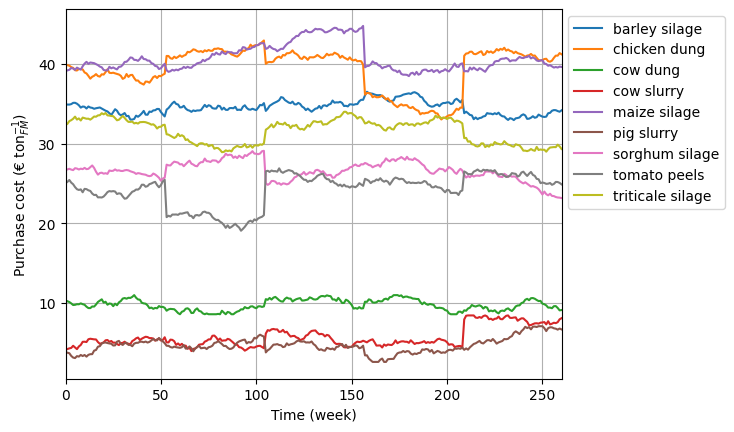
\includegraphics[width=1\columnwidth]{./img/Pricedata_2024-05-07.png}
 \end{center}
 \caption{Generated price data time series for each item}
 \label{fig:dataprice}
\end{figure*}

For a first design of uncertainty, all sources were included in the problem formulation separately, so that 3 different random variables were introduced. Since price and BMP$_\infty$ are very unlikely to be correlated, designing uncertainty separately could be overly conservative (i.e. both taking extreme values for the same realization), but it was reasoanable for first attempts and for being able to assess the sensitivity of J to each of them too. On the other hand, price realizations are likely to have a correlation with item availabilities.
Table \ref{tab:randomvar} reports the same nomenclature that is found in the COLAB to discriminate between the different sources of uncertainty. The uncertainty sets (formalized in Eq.\ref{eq:sets}) were all designed as budgeted sets to avoid being too conservative (es. with box sets). Budgeted was choose over ellipsoidal sets just to preserve the linearity (over convexity) of the robust counterpart. 
The sets are similarly formalized as below for random variable, i.e.:
\begin{equation}\label{eq:sets}
\begin{aligned}
    \mathcal{Z}:=\{z\in\mathbb{R}^n\,|\,z\in[-1,\,1]^n,\|z\|_1 \leq \Gamma_Z\}\,\\
    \mathcal{W}:=\{w\in\mathbb{R}^n\,|\,w\in[-1,\,1]^n,\|w\|_1 \leq \Gamma_W\}\,\\
    \mathcal{L}:=\{l\in\mathbb{R}^n\,|\,l\in[-1,\,1]^n,\|l\|_1 \leq \Gamma_L\}\,
\end{aligned}
\end{equation}
% Table generated by Excel2LaTeX from sheet 'For Report'
\begin{table*}[htbp]
  \centering
  \caption{Nomenclature as present in COLAB for the different uncertanity sources}
    \begin{tabular}{SlScScSc}
    \toprule
    Source of uncertainty & Random variable & Uncertanty Set & Set size parameter \\
    \midrule
    Availability & z     & availabilitySet     & Gamma\_availability \\
    Prices & w     & pricesSet     & Gamma\_price \\
    BMPinf & l     & BMPSet     & Gamma\_BMP \\
    \bottomrule
    \end{tabular}%
  \label{tab:randomvar}%
\end{table*}%
The size parameter was firstly calibrated in order for $\mathcal{Z,W}$ and $\mathcal{L}$ to be such that a robust linear constraint employing $z,w$ or $l$ is guaranteed to satisfy the chance constraint with Prob\% (95\%) probability (Theorem 3.2 of lecture notes).

As shown in Fig.\ref{fig:distribdata}, the generated price data were not symmetric, so that Theorem 3.5 of the lecture notes could not apply. For this reason, it was chosen to design the size parameters based on the actual distribution of data.

\begin{figure*}[htb]
 \begin{center}
  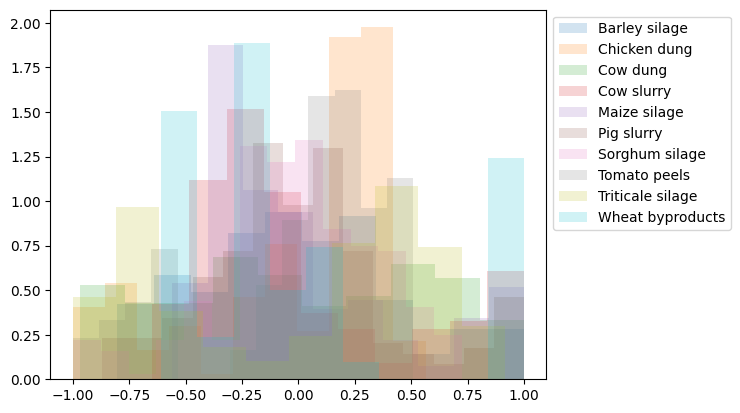
\includegraphics[width=1\columnwidth]{./img/Distribution_price_2024-05-06.png}
 \end{center}
 \caption{Histograms of $Z_P$ for each item}
 \label{fig:distribdata}
\end{figure*}

Data were first standardized as for Eq.\ref{eq:standardize} to be consistent with the definition of random variables as "perturbation" with respect to the mean values, i.e.:
\begin{equation}\label{eq:standardize}
\begin{aligned}
    R_A = \mu_A +P_A Z_A, \\
    R_P = \mu_P +P_P Z_P
\end{aligned}
\end{equation}
where $\mu$ contains the mean realizations, $P\in \mathbb{R}^{n \times n}$ are diagonal matrices containing the maximum deviations, $Z_A \in \mathbb{R}^{n \times 5}$ and $Z_P \in \mathbb{R}^{n \times 260}$ are the matrices that contain all the standardized realization of availabilities and prices respectively.
The latter were thus sorted based on their norm-one; the value that corresponded to the desired P was considered as $\Gamma_Z$ and $\Gamma_W$. 
It is noteworthy to highlight that, due to the very few realizations of availability, the design of $\Gamma_Z$ was very much impacted by rounding in quantizing the sorted realizations.

The size of the uncertainty set for BMP$_\intfty$ was computed as suggested by Theorem 3.5:
\begin{equation*}
   \Gamma_L = \sqrt{2 n \log_{10} \frac{1}{1-P}} 
\end{equation*}
%------------------------------------------------------------------
\subsection{R-LP formulation}
Because of two sources of uncertainty being present in the formulation of \emph{J}, the latter was re-written in forms of two inequality constraints on revenues and operational expenditures.
The robustifed problem ('R-LP') was thus formulated as:
\begin{eqnarray*}
\max_{x\in\chi,s,c}&&J=s-c\\
\mbox{s.t.} && s \leq \sum_{i=1}^{n}\sum_{j=1}^{m} p_{ch4} BMP_{i} VS_{i} \frac{x_{i,j}}{N} \forall l=1,\dots,L\\
&& c \geq \sum_{i=1}^{n}\sum_{j=1}^{m} (C_{Pi,j} +C_{Ti,j})\frac{x_{i,j}}{N}\forall z=1,\dots,Z\\
&& \frac{\sum_{j=1}^{m}\sum_{i=1}^{n\in R} x_{i,j}}{\sum_{j=1}^{m}\sum_{i=1}^{n} x_{i,j}} \lessgtr RL_{r} \ \forall r=1,\dots,R\\
&& x_{i,j} \leq A_{i,j} \ \forall i=1,..,n,\ \forall j=1,..,m,\ \forall w=1,..,W\\
&& k_{min}\leq \frac{\sum_{i=1}^{n}\sum_{j=1}^{m} k_i x_{i,j}}{\sum_{i=1}^{n}\sum_{j=1}^{m} x_{i,j}}\leq k_{max}\ \forall k=1,\dots,K\,\\
&& \frac{\sum_{i=1}^{n}\sum_{j=1}^{m} (BMP_{\infty,i}-BMP_{i}) x_{i,j}}{\sum_{i=1}^{n}\sum_{j=1}^{m} BMP_{i} x_{i,j}}\leq BMP_{res,max}\\\
&& HRT = \frac{V_RN}{\sum_{i=1}^{n}\sum_{j=1}^{m} x_{i,j}}\\
&& x_{i,M} = A_{i,M}\ \forall i=1,\dots,n\\
&& x_{i,j}\geq 0\ \forall i=1,\dots,n\ \forall j=1,\dots,m\\
\end{eqnarray*}

In the formulation above, the following equalities hold:
\begin{eqnarray*}
BMP(HRT,l) = && \overline{BMP(HRT)}\left(1+\left(1-\frac{BMP_{\infty,min}}{\overline{BMP_{\infty}}}\right)l\right ),\\
BMP_{\infty}(l) = && \overline{BMP_\infty}\left(1+\left(1-\frac{BMP_{\infty,min}}{\overline{BMP_{\infty}}}\right)l\right ),\\
C_P(w) = && bm(\mu_{P} +P_{P} w),\\
A(z) = && (ss^T(\mu_A +P_A z))^T
\end{eqnarray*}
where $bm$ is the binary matrix than indicates the presence of the items at the sellers, $ss$ is a matrix that indicates the re-partition of the overall items availability as proportional to the different seller "sizes" and $\overline{BMP(HRT)}, \overline{BMP_{\infty}}$ are the deterministic values of the conversion yield at the given HRT and the maximum achievable, respectively.

The hard constraint that forces the consumption of what is produced by the plant itself (\emph{j=M}) could not be easily robustified, so that it was left as in the deterministic form (the plant manager is fairly more confident on its own plant future production).
\section{Results}
%Maintain past tenses for results obtaiend!!

\subsection{Deterministic LP}
The simplified approach represented nothing but a upper-bound of the more realistic one. Indeed, as HRT was computed from the results of the simplified-LP, the constraint for HRT$_{min}$ was always active (the higher the inflow rate, the higher the profit if no realistic worsening effects on the productivity resulting from a low HRT are considered).
It was interesting to note that, running the realistic-LP with HRT=$+\infty$, the solution suggested the same diet of the simplified-LP, whereas setting HRT=HRT$_{min}$ the suggested diet was different.
It can be concluded, as expected, that the diet with the highest conversion yield (i.e. BMP$_\infty$) is different from the one with the highest productivity (i.e. BMP at low HRT values), and that, under realistic approach, the profit was maximized adopting the one with the highest productivity.
As a result, the best profit was always obtained at the lowest feasible HRT (19 days), and that the latter may be higher only in case the constraint on BMP$_{res,max}$ is active and more restrictive (or similarly, some other possible constraints to avoid excessive residual organic matter in the effluent or the risk for reactor acidification). If no direct/indirect bounds on HRT is enforced, the best profit was achieved for HRT=4, that would for sure lead to reactor acidification, bacteria inhibition and consequent drop of the productivity (verification with ADM1).
This is due to the fact that, with the collected data and related BMP(HRT) curves, the objective function value was more sensitive to the quantity of purchased material than to the conversion yields, in the HRT range of practical interest. 
It is also important to highlight that the other operational expenditures that were neglected are inversely proportional to HRT (es. pumping cost, heating self-consumption, costs of digestate valorization or disposal).
Eventually, from expert knowledge we can state that the most interesting region for real plant operation is between 30-40 days.

Results from multiple realistic-LP runs at different HRT suggested a relevant and superlinear decrease in the profit with HRT, and an interesting shift in the diet composition, as shown in  Fig.\ref{fig:screeningHRTD}. 
In the HRT range of interest, 'maize silage' was the best cost-effective item to select, as also suggested by Fig.\ref{fig:netprofitbmp}. The extent of selection of 'maize silage' was defined by the feasible region, limited by the infleunt diet process and regulating authority constraints. In this case, 'maize silage' was always selected at the highest extension up to the 20\% regulating authority limit. At low HRT values, the extent of carbon-rich items in the diet was higher (+34.6\%) with respect to high HRT values. As they are characterized by faster degradation kinetic and higher BMP$_\infty$ with respect to slurries, this increased even further the difference between J values for low/high HRTs. Barley and triticale silages are thus selected to reach the upper limit on the exploitation of agri-products (P). 
It is important to highlight that slurries and dungs (S category) are forced to constitute a big percentage of the diet to fulfill both VS and regularing authority constraints ($\geq$ 70\%). Slurries are preferred over dungs because of their lower VS content: indeed, dungs present a conversion yield similar to slurries but with higher VS content that would limit the selection of silages, that are charcterized by higher unitary profit as shown in Fig.\ref{fig:netprofitbmp}.
It was interesting to note the shift from pig to cow slurry with increasing HRT: 'cow slurry' is more expensive, but it has also a higher BMP$_\infty$. 
Where possible, the problem tent to push toward the purchase of silages, and fulfill the other constraints with the more productive 'cow slurry'. Nevertheless, at high HRT, silages purchase was limited by the VS constraint on the diet: indeed, cow has higher VS content than pig slurry. In addition, the fixed amount of constrained 'cow dung' produced at the plant characterized by relatively high VS has a higher impact on this constraint at high HRT.
At low HRT the purchased quantities must be higher, so that it was chosen to move to the cheaper and lower-productive pig slurry and, thanks to the higher room for VS, increase the content of silages in the diet. 
Altought silages are more cost-effective than slurries, the J tent to be sensitive to slurries because their extent in the diet is forced to be always much higher than the other items for the VS and regulating authority constraints. The exploitation of other promising substrates such as 'wheat byproducts' and 'chicken dung' is probably hindered by their high TKN value.
Indeed, we remark that the active technical constraints are the VS (for all HRT values) and the TKN (for intermediate HRT values) ones.

Interestingly, intermediate HRTs result in a higher degree of diversification between the two slurries.

All the considerations based on the analysis of Fig.\ref{fig:netprofitbmp} are consistent also because of the small relevance of transportation costs in the distance range that was considered (0-50 km): indeed, they made up between 17-18\% of the total costs for all the HRT values. If the best items as identified by Fig.\ref{fig:netprofitbmp} were present only at very far away locations or if they were characterized by very high specific fixed transportation tariff, the considerations must be re-discussed. 

\begin{figure*}[htb]
 \begin{center}
  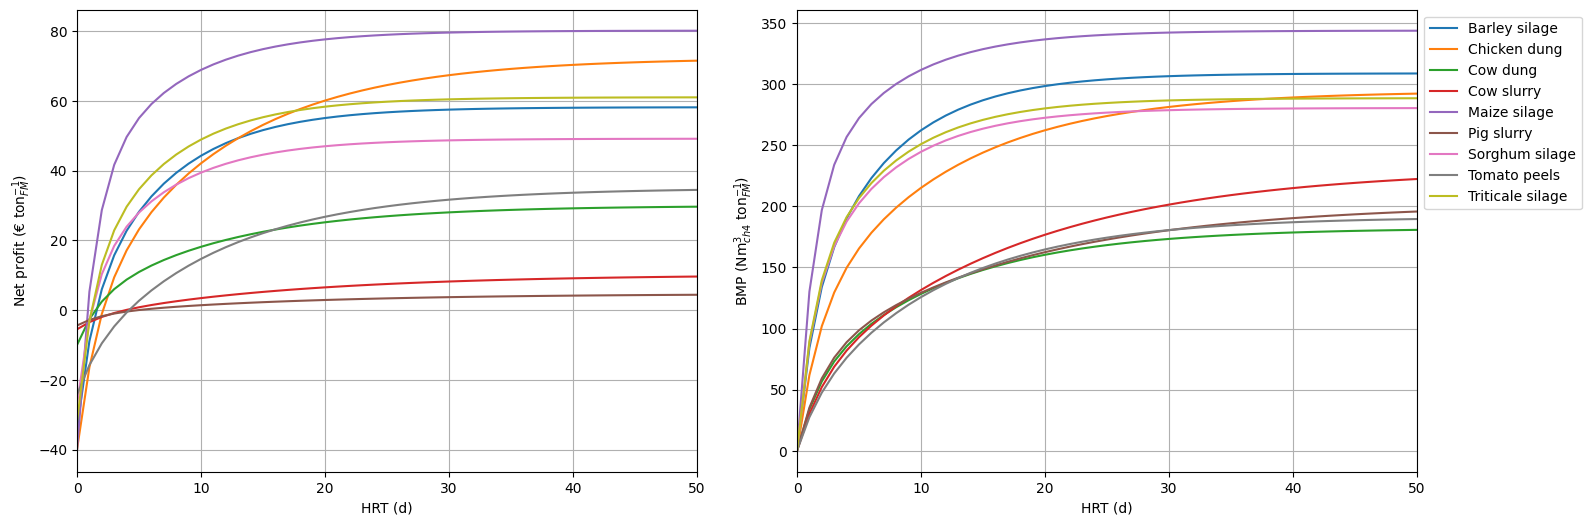
\includegraphics[width=2\columnwidth]{./img/NetProfitBMP_2024-05-02.png}
 \end{center}
 \caption{Comparison between the specific unitary profit (left) and BMP (right) of the different items. Here, the profit does not consider the transportation cost. 'Wheat by-products' is not shown, because out from the scale of interest. Unitary profit was computed as $p_{ch4} \times VS \times BMP(HRT) - C_p$}
 \label{fig:netprofitbmp}
\end{figure*}

\begin{figure*}[htb]
 \begin{center}
  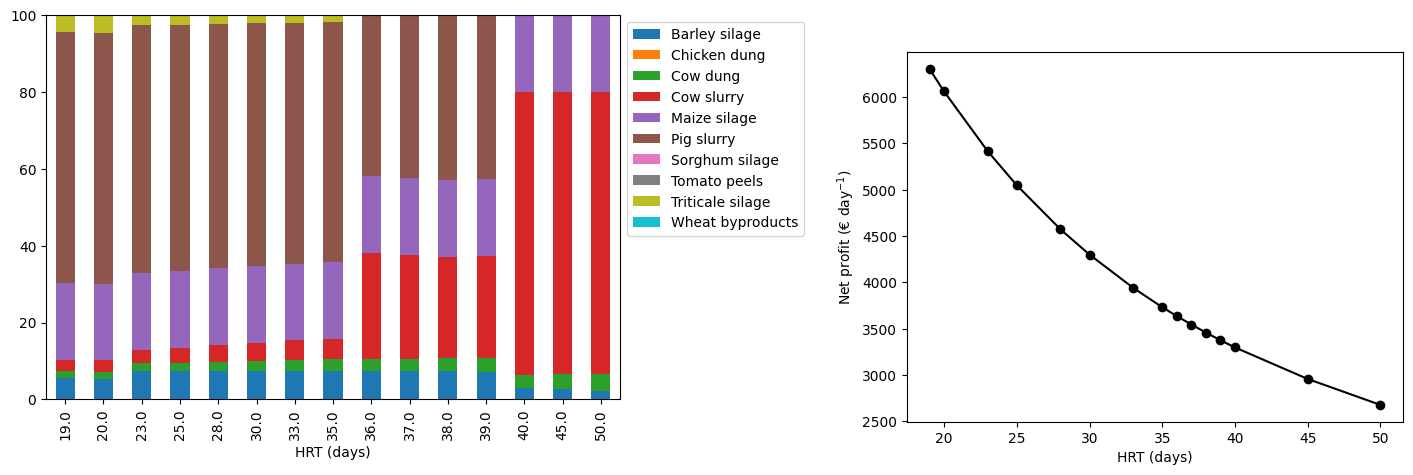
\includegraphics[width=2\columnwidth]{./img/Screening_HRT_D-LP_2024-05-02.png}
 \end{center}
 \caption{Comparison between LP solutions (left) and objective function values (right) obtained for different value of HRT}
 \label{fig:screeningHRTD}
\end{figure*}
%------------------------------------------------------------------------------------

\subsection{Robustified (R-) LP}

The introduction of availability uncertainty is not of particular interest, as the worst-case scenario for the problem under study is very likely to coincide to a realization for which all the item availabilities are equal to their lower-bound i.e. to a deterministic formulation with new bounds to matrix \emph{A}. As few of the availability constraints were active, enforcing uncertainty did not affect significantly the value of the profit ($\leq$ 1\%): this was due to the low impact of transportation costs for the less abundant and interesting items (i.e. silages), coupled with a small difference between transportation costs of the nearest and the second-nearest sellers. The impact could be more relevant for if data are generated with higher variance. The only difference in the diet composition was observed at low HRT, with a reduced purchase of 'triticale silage', substituted by 'barley silage' (triticale is slightly more cost-effective, but with a higher VS content).

The introduction of price uncertainty did impact the value of the profit of 14.4\% and 13.8\% for HRT equal to 20 and 50 respectively. Interestingly, the diet remained almost the same as for the deterministic solution, proving resiliance to price uncertainty of the optimal diet.

Similar considerations hold if only BMP$_\infty$ (and availability) uncertainty is introduced, although a higher impact was observed, as the profit dropped by 30.1\% and 26.9\% for HRT equal to 20 and 50 respectively.

When the two uncertainty sources were simultaneously introduced, the profit dropped by 44.5\% and 40.6\% for HRT equal to 20 and 50 respectively. This may suggest that operating a reactor with high HRT is only slightly more robust. Nevertheless, the absolute profit loss introduced by robustification is much higher for a rector with low HRT (148\%). 
It is important to note that the worst-case realization at HRT=20 still returned a slightly higher profit then the deterministic profit at HRT=50.

At HRT=50, some 'maize silage' was substituted with 'barley silage': this is most likely due to the higher maximum/mean ratio of the price of maize with respect to barley. It can be stated that barley is the safest alternative to maize.

The results of the screening for different HRT values screening are shown in Fig.\ref{fig:screeningHRTR}.
The standard deviation computed on the same HRT values for both the LP and R-LP J values suggested a lower variability (-28.6\%) with HRT for the robustified solutions. This also increases the "degree of robustness" of the solution obtained with the R-LP formulation. 

The differences in the diet compositions follow similar considerations as for the LP solutions was confirmed (es. barley as second-best and safer alternative to maize at high HRTs).
Nevertheless:
\begin{itemize}
    \item The shift from pig to cow slurry is moved to lower HRTs. Indeed, 'cow slurry' is a safer option than 'pig slurry' because of its lower max/mean ratio of the purchase price and higher min/mean ratio of the BMP$_\infty$;
    \item Less 'triticale silage' is available for purchase at low HRTs.
\end{itemize}

The values of the "nominal" size parameters for the uncertainty sets are reported in Table. 

\begin{figure*}[htb]
 \begin{center}
  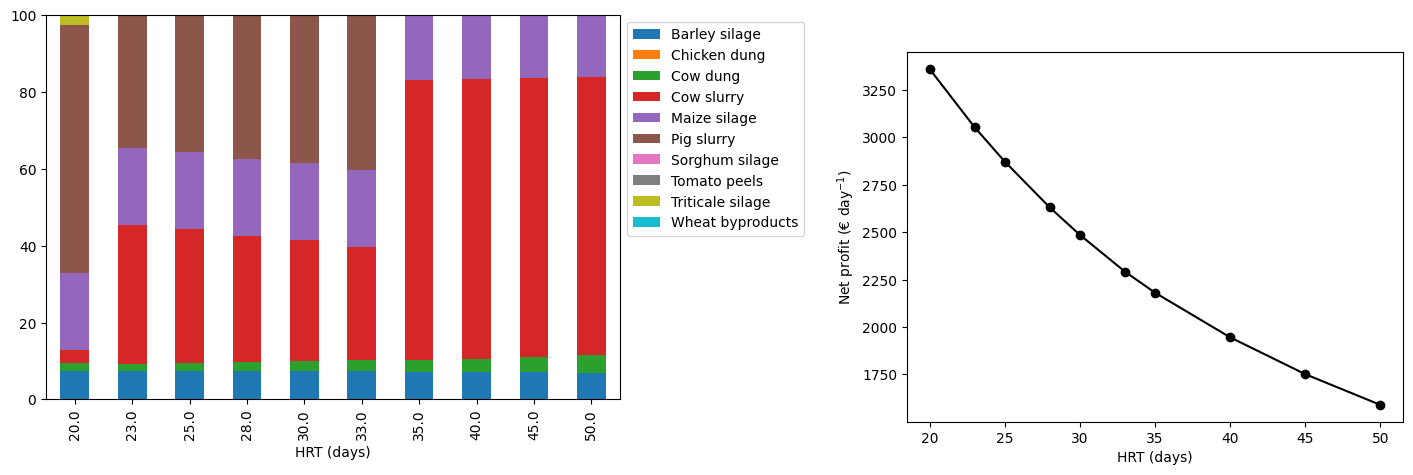
\includegraphics[width=2\columnwidth]{./img/Screening_HRT_R-LP_2024-05-02.png}
 \end{center}
 \caption{Comparison between R-LP solutions (left) and objective function values (right) obtained for different value of HRT}
 \label{fig:screeningHRTR}
\end{figure*}

After the model was solved with the "nominal/trained" value of Gamma\_price, some later testing was performed. Additional realization of price data were generated for the consequent remaining 20 years of future plant operation. For each realization, the value of J was computed taking the same values of decision variables obtained so far, for both a high and low HRT value (50 and 20 days respectively). The "nominal" J value was compared with the distribution of J obtained under testing price realizations and results are shown in Fig.\ref{fig:testing20}-\ref{fig:testing50}. It is important to stress out that this comparison was possible only under the same realization of availability and BMP$_\infty$: in this case, the deterministic values were considered.
The profit of the deterministic LP was found in line with the ones computed under testing realizations; nevertheless, it was slightly too optimistic, being higher than the average profit obtained in testing (few percentage points).
In contrary, the profit suggested by the R-LP looks overly conservative, being 11.9\% and 11.1\% lower than the profit value located at the "minimum" whisker of the box-plot, for HRT=20 and 50 respectively. 
From the width of the box-plots, it was also interesting to note the greater dispersion of the profit values at HRT=20 with respect to HRT=50, remarking the higher "safety degree" of reactors operated at high HRTs. 

\begin{figure}[htb]
 \begin{center}
  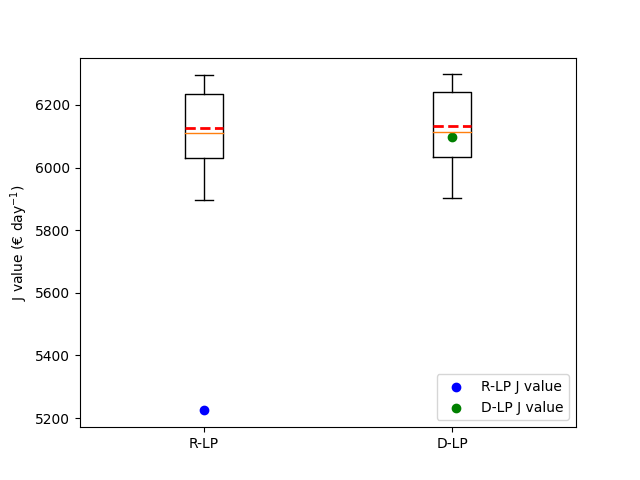
\includegraphics[width=1\columnwidth]{./img/Testing_20_2024-05-02.png}
 \end{center}
 \caption{Comparison between nominal and test objective function value for HRT=20}
 \label{fig:testing20}
\end{figure}

\begin{figure}[htb]
 \begin{center}
  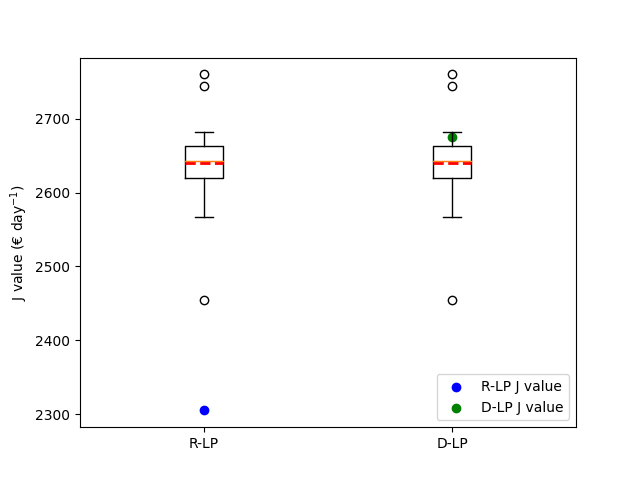
\includegraphics[width=1\columnwidth]{./img/Testing_50_2024-05-02.png}
 \end{center}
 \caption{Comparison between nominal and test objective function value for HRT=50}
 \label{fig:testing50}
\end{figure}
%------------------------------------------------------------------------------------

%\subsection{Unique $\mathbf{\Zeta}$ vs multiple $\Zeta$'s}
%------------------------------------------------------------------------------------

\subsection{Map of optimal solutions for different $\Gamma$}

Some analysis was carried out to assess the impact of the choice of the size parameters for the uncertainty sets. The aim was to provide decision-makers a map of the possible worst-case profits and diet compositions under different "risk degree" (Prob parameter). Table\ref{tab:gammas} reports the values investigated and the consequent values of the size parameters. The number of items that can simultaneously attain extreme values is highly impacted by the value of Prob, in particular for the BMP$_\infty$, coherently with the higher dispersion that Theorem 3.5 covers with respect to the lower variance of the availability and price distributions. 

Results are reported in Fig.\ref{fig:screenVaR20}-\ref{fig:screenVaR50}.

As far as the comparison between low and high HRT is concerned, the same observations on the higher variability of the profit with low HRT held.
Additionally, interesting differences in the diet composition were observed:
\begin{itemize}
    \item At high Prob, the value of the size parameters was bigger than the number of different items present in the diet. In the worst-case realization, both slurries could be at their worst performance (high price and low BMP$_\infty$), so that the one leading to the best worst-case was selected to cover all the diet percentage imposed by VS and regulating authority constraints. The choice of pig or cow at the different HRT followed the above-mentioned observations (es. at low HRT I have to buy more, so I choose the cheapest (pig) to fulfill constraints). When the size parameter was bigger than its nominal (Prob=95\%) value, nor J or the diet changed: this was still due to the fact that the size parameter became larger the the number of items present in the diet with in a relevant percentage i.e. able to affect J the most (3 or 4).
    \item At low Prob (Prob $\leq$ 20\% i.e. Gamma\_price $\leq$ 3 and Gamma\_BMP $\leq$ 2), a lower number of items ($\leq$ number of items relevant in the diet composition) could attain its worst-case, so that the tendency of the solver to diversify the diet was clearly observable.
    \item Interestingly, the J value at extremely low Prob is lower with respect to the deterministic profit for the same HRT. This could be partially due to a small deviation of \emph{$\mu_P$} from the deterministic purchase prices, but was primarily due to the relevant value of the price set size parameter (Gamma\_price $\geq$ 1.8). Indeed, this value was high enough to affect at their worst-case the most relevant items in the diet and thus impacting a low the profit.
    In addition, from Fig.\ref{fig:dataprice} we observe the (realistic) low range of variability of 'cow slurry' and 'pig slurry'. Due to this reason, after the most of the profit loss due to price extinguished at low Prob, the impact of only price uncertainty at higher values of Prob did not increases substantially (only 4.3\% profit drop from 1\% to 95\% Prob values, if only price (and availability) uncertainties were in place).
    \textcolor{red}{Consideration of intermediate values leading to more triticale than maize? Intermediate Prob similar to intermediate HRTs?}
\end{itemize}

% Table generated by Excel2LaTeX from sheet 'For Report'
\begin{table}[htbp]
  \centering
  \caption{Uncertainty set size parameters correspondent to different threshold of probability Prob to meet the change constraint}
    \begin{tabular}{ScScScSc}
    \toprule
    Prob & Gamma\_availability & Gamma\_price & Gamma\_BMP \\
    \midrule
    1\%   & 4.7   & 1.8   & 0.4 \\
    5\%   & 4.7   & 2.1   & 1.0 \\
    10\%  & 4.7   & 2.2   & 1.5 \\
    20\%  & 4.7   & 2.7   & 2.1 \\
    30\%  & 5.2   & 3.0   & 2.7 \\
    40\%  & 5.2   & 3.3   & 3.2 \\
    50\%  & 6.3   & 3.7   & 3.7 \\
    60\%  & 6.3   & 4.1   & 4.3 \\
    70\%  & 6.5   & 4.5   & 4.9 \\
    80\%  & 6.5   & 4.7   & 5.7 \\
    90\%  & 7.2   & 5.0   & 6.8 \\
    95\%  & 7.2   & 5.4   & 7.7 \\
    99\%  & 7.2   & 5.9   & 9.6 \\
    \bottomrule
    \end{tabular}%
  \label{tab:gammas}%
\end{table}%


\begin{figure*}[htb]
 \begin{center}
  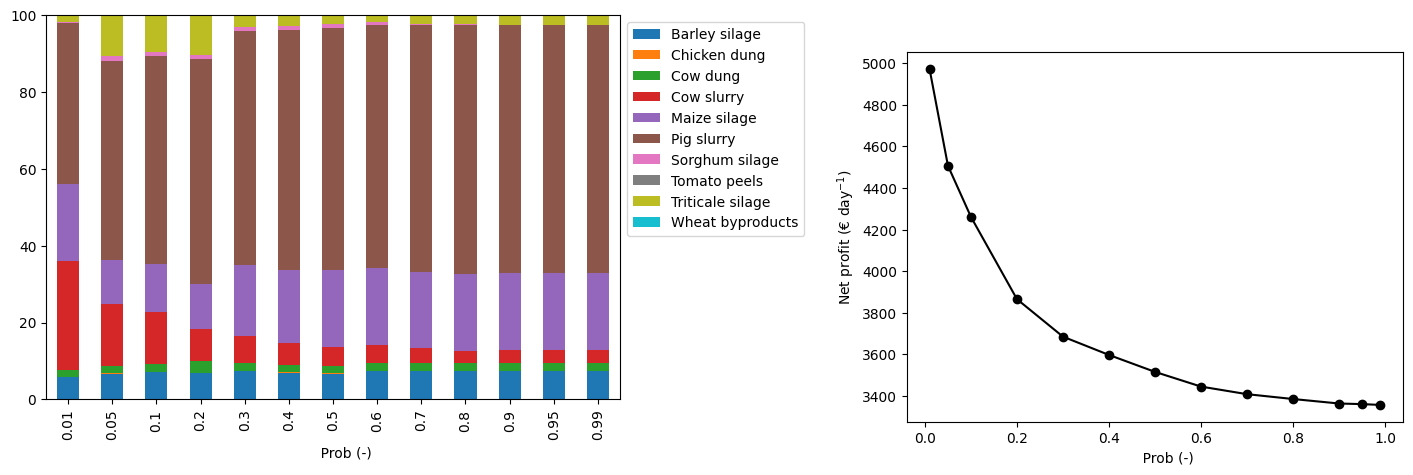
\includegraphics[width=2\columnwidth]{./img/Screening_VarProb_R-LP_20_2024-05-02.png}
 \end{center}
 \caption{Comparison between solutions (left) and objective function values (right) obtained for different value of confidence interval (VaRProb) and HRT=20}
 \label{fig:screenVaR20}
\end{figure*}

\begin{figure*}[htb]
 \begin{center}
  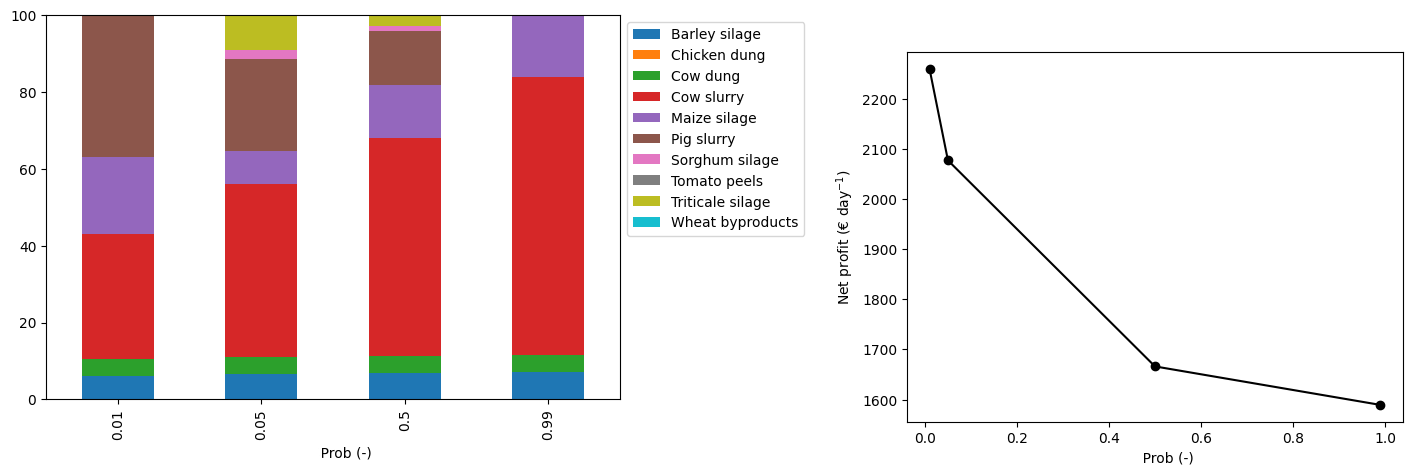
\includegraphics[width=2\columnwidth]{./img/Screening_VarProb_R-LP_50_2024-05-02.png}
 \end{center}
 \caption{Comparison between solutions (left) and objective function values (right) obtained for different value of confidence interval (VaRProb) and HRT=50}
 \label{fig:screenVaR50}
\end{figure*}

%------------------------------------------------------------------------------------

\subsection{Conclusions and further improvements}
\begin{itemize}
    \item For the case under study and with the boundary conditions shaped by the considered data, the exploitation of industrial by-products (es. 'tomato peels' and 'wheat byproducts') in the inflent diet of biomethane plants is not favoured.
    \item Other operational expenditures such as energy self-consumption, etc. can be included to result in more accurate predictions of profit and pushing optimality toward higher values of HRT.
    \item High HRT is suggested for case studies surrounded by high uncertainty. On the other hand, low HRT leads to higher profits. Worst-case realizations for low HRT may result in profits similar to the deterministic problem for high HRT. If non-linear process uncertainties are also considered with the aid of ADM1 simulations of the optimal robust diet, low HRT could be robustly applied to the operation of reactors and higher profits could be achieved.
    \item Price and BMP$_\infty$ uncertainties were proved to have a major impact on the achievable profit. Problem robustification was proved to give conservative results and provide the possibility to derive some interesting considerations on the most profitable and the most robust items/diets.
    \item \textcolor{red}{State someway somehow that we were overly conservative with size parameters and how to improve our estime...jointly BMP and price?}
    \item In this demonstrative problem formulation and solution, N was taken equal to one year for simplicity. Nevertheless, a lower N can be set by decision makers: in that case, the availability and price data must conserve their time dimension when designing uncertainty sets. Indeed, the subset of realizations filtered to the time window of the next selected operating horizon (start time and duration) would need to be considered to adapt the worst case solution to crop and market seasonality. 
    \item Better estimation of BMP(HRT) considering a more realistic behaviour of a continuously fed reactor (different from similarity with batch reactor that was made). 
    A more reliable representation of the operating behaviour of a continously-fed reactor could improve the accuracy of the predictions and favour higher HRTs, in comparison to the assumed similarity with batch-tests for the productivity estime.
    Indeed, instead of Eq.\ref{prodbatch}, Eq. \ref{prodcont} should be used, i.e.
\begin{equation}\label{prodbatch}
    Q_{ch4,i} = BMP_i(HRT) \frac{x_i}{N}
\end{equation}
\begin{equation}\label{prodcont}
    Q_{ch4} = \frac{x_i}{N} \sum_{t=0}^{HRT} E_{CSTR}(t) BMP_i(t) 
\end{equation}
    where \emph{E$_{CSTR}$(t)} is the fraction of effluent material remained in the reactor until time t.
    \item A multi-objective approach can guide further the decision of the operating HRT, trading-off the higher profits of low HRTs with the lower profit variability of high HRTs.   
\end{itemize} 

\section{Appendix}
% Table generated by Excel2LaTeX from sheet 'For Report'
\begin{table*}[htbp]
\scriptsize
  \centering
  \caption{Deterministic value of item technical characteristics, fixed tariff for transportation costs and purchase price}
    \begin{tabular}{SlScScScScScScScScScScScSc}
    \toprule
          & Leg. Cluster & TS    & VS    & BMPinf & Fixed\_tariff & TKN   & C/N   & TAN   & TAC   & LI    & TVFA  & Cp \\
    \midrule
          & \multirow{2}[2]{*}{-} & kgTS  & kgVS  & Nm3CH4 & €     & kgN   & molC  & kgN   & kgCaCO3 & kgLI  & kgHAc & € \\
          &       & tonFM-1 & tonFM-1 & tonVS-1 & 20tonFM-1 & tonFM-1 & molN-1 & tonFM-1 & tonFM-1 & tonFM-1 & tonFM-1 & tonFM-1 \\
    \midrule
    Barley silage & P     & 280.0 & 262.4 & 308.8 & 50.0  & 14.0  & 48.8  & 0.5   & 0.0   & 8.4   & 5.6   & 34.0 \\
    Chicken dung & S     & 458.1 & 335.5 & 294.4 & 60.0  & 26.0  & 9.0   & 1.5   & 3.0   & 13.7  & 1.0   & 40.0 \\
    Cow dung & S     & 242.5 & 192.9 & 182.2 & 50.0  & 4.0   & 24.0  & 0.5   & 3.0   & 7.3   & 1.0   & 10.0 \\
    Cow slurry & S     & 71.8  & 59.8  & 231.4 & 60.0  & 3.1   & 18.8  & 1.5   & 10.0  & 3.6   & 5.0   & 5.5 \\
    Maize silage & P2    & 325.3 & 308.0 & 343.7 & 50.0  & 3.7   & 48.8  & 0.5   & 0.0   & 9.8   & 10.0  & 40.3 \\
    Pig slurry & S     & 51.3  & 39.6  & 202.3 & 60.0  & 3.0   & 11.0  & 2.2   & 15.0  & 3.9   & 4.0   & 4.4 \\
    Sorghum silage & P     & 258.5 & 238.7 & 280.4 & 50.0  & 4.0   & 48.8  & 0.5   & 0.0   & 7.8   & 5.6   & 27.0 \\
    Tomato peels & B     & 281.3 & 272.3 & 191.4 & 50.0  & 8.0   & 20.0  & 0.3   & 0.0   & 2.8   & 1.0   & 24.3 \\
    Triticale silage & P     & 300.0 & 283.5 & 288.5 & 50.0  & 4.0   & 48.8  & 0.5   & 0.0   & 9.0   & 5.6   & 32.0 \\
    Wheat byproducts & B     & 884.5 & 833.0 & 331.9 & 50.0  & 22.0  & 54.0  & 0.0   & 0.0   & 34.5  & 1.0   & 153.4 \\
    \bottomrule
    \end{tabular}%
  \label{tab:items}%
\end{table*}%


\addtolength{\textheight}{-12cm}   % This command serves to balance the column lengths
                                  % on the last page of the document manually. It shortens
                                  % the textheight of the last page by a suitable amount.
                                  % This command does not take effect until the next page
                                  % so it should come on the page before the last. Make
                                  % sure that you do not shorten the textheight too much.

%
%%%%%%%%%%%%%%%%%%%%%%%%%%%%%%%%%%%%%%%%%%%%%%%%%%%%%%%%%%%%%%%%%%%%%%%%%%%%%%%%%
%%python look for sampling from triangular distribution

\end{document}
